\documentclass[12pt,letterpaper]{article}
\usepackage[utf8]{inputenc}
\usepackage[margin=1 in]{geometry}
\usepackage{graphicx}
\usepackage{float}
\usepackage{amsmath}
\usepackage{caption}
\usepackage[hidelinks]{hyperref}

\renewcommand{\baselinestretch}{1.5}

\begin{document}

%%%%%%%%%%%%%%%%%%%%%%%%%%%%%%%%%%%%%%%%%%%%%%%%%%%%%%%%%%%%%%%%%%%%%%%%%%%%%%%

% Cover page

\thispagestyle{empty}

\begin{center}

{\Large \textbf{A Report} \\}
\medskip
{\large \textbf{ON} \\} 
\medskip
{\large \textbf{VEHICLE DETECTION ON JETSON NANO}}

\vskip 1.5in

{\large BY}
\bigskip

\addtolength{\tabcolsep}{20pt}
\begin{tabular}{cc}
    {\large Rahul Ganesh Prabhu} & {\large 2018A7PS0193P} \\
    {\large Saurabh Wandhekar} & {\large 2018A7PS0157G}
\end{tabular}
\addtolength{\tabcolsep}{-20pt}

\vskip 1.5in

{\large AT \\}
\medskip
{\large CENTRE FOR DEVELOPMENT OF ADVANCED COMPUTING, PUNE} \\ 
\vskip 0.4in
{\large A Practice School - I Station of} \\
\vskip 0.4in
{\large \textbf{BIRLA INSTITUTE OF TECHNOLOGY \& SCIENCE, PILANI}}
\vskip 0.4in
{\large \textbf{(June,2020)}}

\end{center}

\pagebreak

%%%%%%%%%%%%%%%%%%%%%%%%%%%%%%%%%%%%%%%%%%%%%%%%%%%%%%%%%%%%%%%%%%%%%%%%%%%%%%%

% Title Page

\thispagestyle{empty}

\begin{center}
    { \large \textbf{
    A REPORT \\
    ON \\
    VEHICLE DETECTION ON JETSON NANO
}
    }

\vskip 1in

{\large BY} \\
\bigskip
\begin{tabular}{c c c}
    {\large  Rahul Ganesh Prabhu} & {\large 2018A7PS0193P} & {\large B.E. (Hons.) Computer Science} \\
    {\large  Saurabh Wandhekar} & {\large 2018A7PS0157G} & {\large B.E. (Hons.) Computer Science} \\
\end{tabular}

\vskip 1in

Prepared in partial fulfillment of the \\
Practice School-I Course No.s \\
BITS C221/BITS C231/BITS C241 \\

\bigskip
{\large AT \\
    CENTRE FOR DEVELOPMENT OF ADVANCED COMPUTING, PUNE \\
    A Practice School-I Station of
}

\vskip 1in


{\large \textbf{BIRLA INSTITUTE OF TECHNOLOGY \& SCIENCE, PILANI}}

{\large \textbf{(June, 2020)}}


\end{center}


\pagebreak

%%%%%%%%%%%%%%%%%%%%%%%%%%%%%%%%%%%%%%%%%%%%%%%%%%%%%%%%%%%%%%%%%%%%%%%%%%%%%%%

% Acknowledgements

\thispagestyle{empty}

\begin{center}
    { \Large \textbf{Acknowledgements}}
\end{center}

We would like to take this opportunity to express our heartfelt gratitude to everyone who has supported us in our work during the course of this project. Firstly, we would like to thank BITS Pilani and CDAC, Pune for giving us a platform in the form of PS-1 to work on this project. 

Further, we would like to thank Rahul Dangi, our mentor for his guidance and for providing us, this opportunity to work under him. He provided us with tremendously valuable resources in order to help us gain deep insight into this project. He has always been keen on helping us by solving our doubts through continuous interactions. We are grateful to him for the same. 

We would also like to thank our faculty mentor, Dr. Tathagata Ray for his continuous motivation and support. He has been guiding us constantly so that we maintain discipline in our work and make the best out of this opportunity. We are thankful to him for the same.

\pagebreak

%%%%%%%%%%%%%%%%%%%%%%%%%%%%%%%%%%%%%%%%%%%%%%%%%%%%%%%%%%%%%%%%%%%%%%%%%%%%%%%

% Abstract

\thispagestyle{empty}

\begin{center}
    {\large 
    \textbf{BIRLA INSTITUTE OF TECHNOLOGY \& SCIENCE, PILANI} \\
     \textbf{(RAJASTHAN)} \\
     \textbf{Practice School Division}
}
\end{center}

\noindent \textbf{Station:} Centre for Development of Advanced Computing, Pune

\noindent \textbf{Duration:} 6 weeks \hfill \textbf{Date of Start:} 18th May, 2020

 \noindent \textbf{Date Of Submission:} 24th June, 2020

 \noindent \textbf{Title of Project:} Vehicle Detection on Jetson Nano

\medskip

\begin{tabular}{c c c}
\textbf{Student Name} & \textbf{ID No.} & \textbf{Discipline} \\
Rahul Ganesh Prabhu & 2018A7PS0193P & B.E. (Hons.) Computer Science \\
Saurabh Wandhekar & 2018A7PS0157G & B.E. (Hons.) Computer Science
\end{tabular}

\medskip

 \noindent \textbf{Name of Mentor:} Rahul Dangi

 \noindent \textbf{Name of PS Faculty:} Dr. Tathagata Ray

 \noindent \textbf{Key Words:} Real-time object detection, resource constrained hardware

 \noindent \textbf{Project Areas:} Object detection, machine learning, neural networks

 \noindent \textbf{Abstract:}

\noindent The goal of this project is to develop an end-to-end machine learning pipeline for the purpose of real-time vehicle detection on resource-constrained hardware like the NVIDIA Jetson Nano. It also involves testing multiple different object detection algorithms to find the best approach for the specified use case. This pipeline will be part of a license plate recognition system for roads and highways.


% TODO: Add more spacing, or maybe add the signatures

\pagebreak

%%%%%%%%%%%%%%%%%%%%%%%%%%%%%%%%%%%%%%%%%%%%%%%%%%%%%%%%%%%%%%%%%%%%%%%%%%%%%%%

% Table of Contents

\thispagestyle{empty}

\tableofcontents

\pagebreak

%%%%%%%%%%%%%%%%%%%%%%%%%%%%%%%%%%%%%%%%%%%%%%%%%%%%%%%%%%%%%%%%%%%%%%%%%%%%%%%

% Content starts

\setcounter{page}{1}

\section{Introduction}

    Object detection is a computer vision task that involves detecting instances of objects of a certain class (e.g. humans, cars, phones) from images or videos. These classes are identified by means of the special visual features they possess, which help us distinguish them from other objects. For example, pedestrians possess facial features like a nose, a mouth and eyes that distinguish them from a bird, which could be distinguished with its beak. Object detection is usually done by employing deep convolutional neural networks for feature extraction, stacked below fully connected layers for classification.

    The Jetson Nano is a small, powerful computer used for embedded applications. It’s spec sheet can be found in Appendix A. It comes equipped with a GPU which is ideal for neural-network-based tasks due to their high throughput, aiding in large matrix operations. However, it still poses a tight resource constraint. Our goal is to process real-time video footage at about 20 frames per second (FPS), but this will not be possible using more complicated networks that use over 100 layers, like YOLOv4. Hence, it is necessary to use lighter object detection models that can run comfortably on embedded hardware. 

For this project, we decided to test and compare two different object detection methods - Tiny YOLOv3 (tested by Rahul Ganesh Prabhu) and SSD Mobilenetv2 (tested by Saurabh Wandhekar). While Tiny YOLOv3 is much lighter, SSD Mobilenet has empirically been found to have a better speed vs accuracy trade-off.


\section{YOLO - You Only Look Once}

YOLO, which stands for You Only Look Once is a fast and accurate real-time object detection system. The first of its kind, it works much faster than older region proposal based techniques like R-CNN. While the region proposal based approaches involve proposing hundreds of “regions” which are processed individually by the convolutional neural network, YOLO processes an image in a single pass. This results in much faster evaluation, making it far more suitable for real-time purposes.

\subsection{How does it work?}

YOLO first divides an input image into an SxS grid. Each grid cell predicts a fixed number of bounding boxes, such that their center lies within the grid cell. However, each grid cell only detects a single object. Every predicted boundary box has its own box confidence score, which defines how confident the neural network is that the bounding box is correct and that it contains an object. Every grid cell also produces different class probabilities, one for every class. These define how probable it is that a given grid cell contains an object of the given class. In practice, only those boundary boxes are chosen whose box confidence scores cross a certain threshold value, which is different depending on the use case.

    This approach faces two problems. For one, if two objects’ centres are within the same grid cell, they cannot be separately detected, since each grid cell produces only one bounding box. The other problem is that it could produce duplicate detection of the same object. In order to mitigate this problem, an algorithm called non-maximal suppression (NMS) is used. It removes duplicate bounding boxes by removing the ones which have a large area of intersection with other bounding boxes that have a higher box confidence score.

\subsection{How are bounding boxes predicted?}

The YOLO network outputs a set of bounding boxes for each grid cell. If YOLO had to predict the dimensions of the bounding boxes as well, training would be very unstable. To make this process easier, we provide “anchor boxes” or “priors”. These anchor boxes are tuples of width and height, that are used to predict the boundary boxes for the different objects in a picture. YOLO does this by predicting offsets to these boxes. These offsets are constrained by a sigmoid function, which keeps the offsets in a [0,1] range, preventing large changes and keeping training stable.

The anchor boxes have to be hand-picked for the given task, as the dimensions of the desired box depends entirely on the dimensions of the desired detections. The desired anchor boxes are generated using k-means clustering. However, using k-means clustering with the Euclidean distance metric empirically leads to favouring larger boxes over smaller ones. To alleviate this, we use a different distance operator that is ubiquitous in object detection - Intersection Over Union (IOU). IOU of two boxes is defined as the ratio of area of their intersection to the area of their union.

\[ IOU = \frac{Area\;of\;Intersection}{Area\;of\;Union} \]

The more two bounding boxes overlap, or in other words, the more alike they are, the higher is the IOU. The results of the clustering can be seen below:

    \begin{figure}[h!]
        \centering
        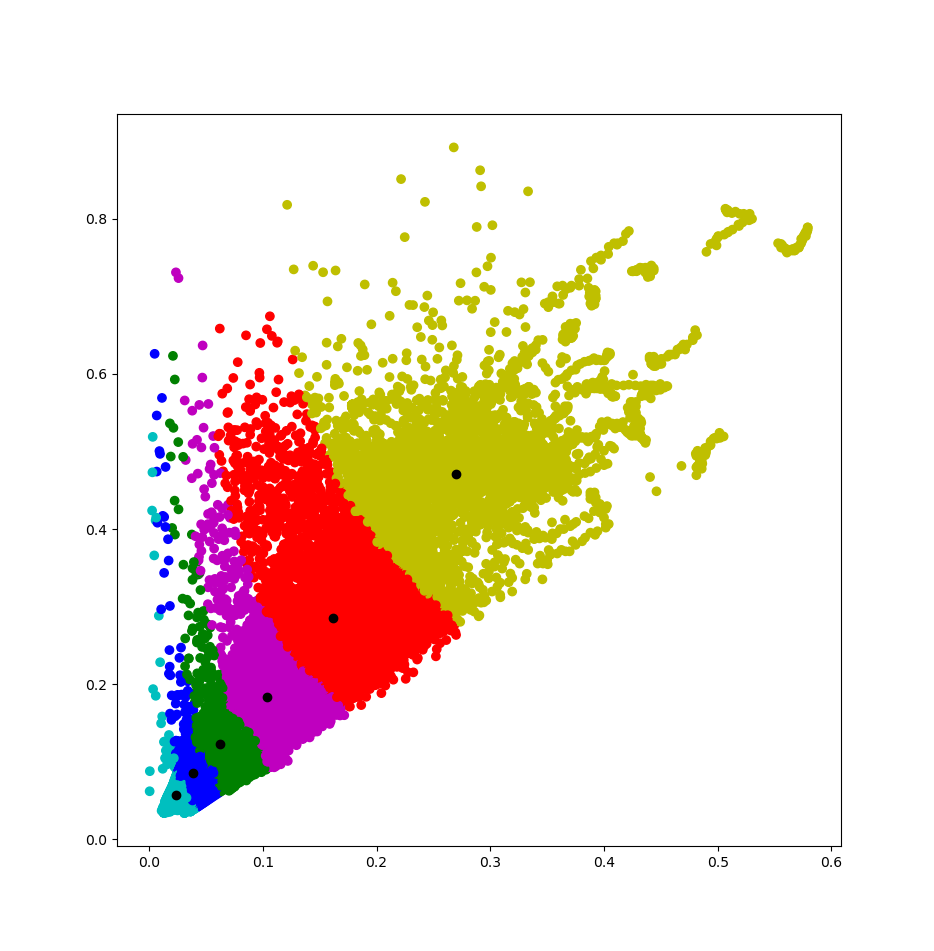
\includegraphics[width=0.8\textwidth,keepaspectratio]{assets/plot.png}
        \caption{Bounding box clustering results}
    \end{figure}

All points of a single colour are in one cluster, while the black dots signify their centres, which are chosen as anchor boxes.

\subsection{The Loss Function}

The YOLO loss function is a sum of three parts:

\begin{enumerate}
    \item Classification Loss: If an object is detected, the classification loss at each cell is the squared error of the class conditional probabilities for each class. The formula is defined below:
        \[ \sum_{i=0}^{S^2} 1_{i}^{obj} \sum_{c \in classes} (p_{i}(c)-\widehat{p_{i}}(c))^2 \] 
    where $1_{i}^{obj} = 1$ if an object appears in cell $i$, otherwise 0

    $\widehat{p_{i}}(c)$ denotes the conditional class probability for class $c$ in cell $i$

\item Localization Loss: This measures the errors in the predicted boundary box locations and sizes. The formula is as defined below:
    
    \[ \lambda_{coord}\sum_{i=0}^{S^2} \sum_{j=0}^{B} 1_{ij}^{obj} [(x_{i} - \widehat{x}_{i})^2 + (y_{i} - \widehat{y}_{i})^2]\; + \; \lambda_{coord}\sum_{i=0}^{S^2} \sum_{j=0}^{B}1_{ij}^{obj}[(\sqrt{w_{i}} - \sqrt{\widehat{w}_{i}})^2 + (\sqrt{h_{i}} - \sqrt{\widehat{h}_{i}})^2 ]    \]

where

$1_{ij}^{obj} = 1$ if the $j^{th}$ boundary box in cell $i$ is responsible for detecting the object, otherwise 0.

$\lambda_{coord}$ increases the weight of the localization loss in the total loss


\item Confidence Loss: If an object is detected in the box, the confidence loss is as defined below:

    \[ \sum_{i=0}^{S^2} \sum_{j=0}^{B} 1_{ij}^{obj} (C_{i} - \widehat{C}_{i})^2 \]

    where

    $\widehat{C}_{i}$ is the box confidence score of the box j in cell i

    $1_{ij}^{obj} = 1$ if the $j^{th}$ boundary box in cell $i$ is responsible for detecting the object, otherwise 0.

    If an object is not detected in the box, the confidence loss is defined as:

    \[ \lambda_{noobj} \sum_{i=0}^{S^2} \sum_{j=0}^{B} 1_{ij}^{noobj} (C_{i} - \widehat{C}_{i})^2  \]

    where

    $1_{ij}^{noobj}$ is the complement of $1_{ij}^{obj}$

    $\widehat{C}_{i}$ is the box confidence score of the box $j$ in cell $i$

    $\lambda_{noobj}$ weighs down this element of the loss, since most bounding boxes do not contain any objects

\end{enumerate}

\subsection{Network Architecture}

YOLOv3 uses a 53-layer Darknet-53 feature extractor, upon which another 53 layers are stacked for the purpose of detection, coming to a total of 106 layers. This is far too much for our embedded system use case. Instead, we use a smaller, lighter model, Tiny YOLOv3.  It uses only 23 layers, making it perfect for our case. The network architecture is as tabulated below:

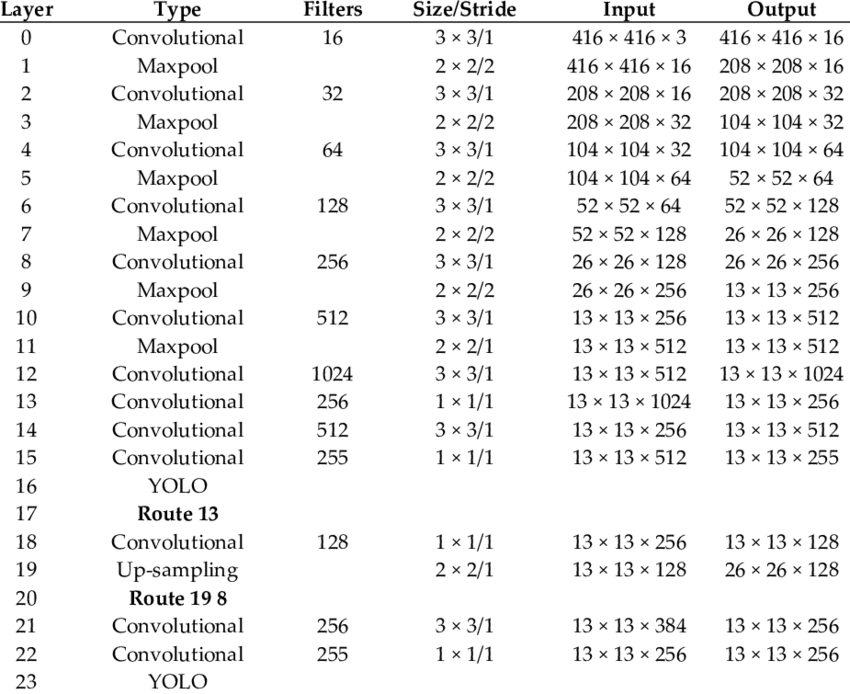
\includegraphics[width=\textwidth,keepaspectratio]{assets/darknettable.png}

\section{SSD - Single Shot Multibox Detector}

SSD is a fast and accurate real-time object detection system. SSD predicts bounding boxes and classes directly from feature maps in one single pass. Feature maps are a representation of the dominant features of the image at different scales. For example, feature maps can be 8x8 or 4x4 grids.

\subsection{How does it work?}

SSD only needs an input image and the corresponding ground truth boxes for each object in the image during training. The model takes an image as input which passes through multiple convolutional layers with different sizes of filters (10x10, 5x5 and 3x3) whose outputs are feature maps. These feature maps from convolutional layers at different positions of the network are used to predict the bounding boxes. We associate a set of default bounding boxes called anchors or priors with each cell of the feature map. These bounding boxes have different sizes and aspect ratios. For each default box, we predict both the shape offsets (width and height) and the confidences for all object categories. At training time, we match these default boxes to the ground truth boxes. For example, in the feature maps below, we have matched two default boxes with the cat and one with the dog, which are treated as positives and the rest as negatives. The chosen boundary boxes are those whose box confidence scores cross a certain threshold, which is different depending on the use case. The non-maximal suppression method is also used at the end of the SSD model to keep the most relevant bounding boxes.

\begin{figure}[h!]
    \centering
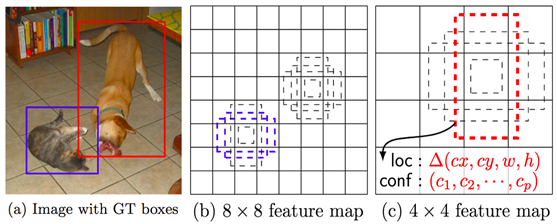
\includegraphics[width = \textwidth,keepaspectratio]{assets/SSDpic.png}
\caption{TODO: Ask Saurabh}
\end{figure}

SSD makes far more predictions than the number of objects present. So, there are many more negative matches than positive matches. This creates a class imbalance that hurts training. We are training the model to learn background space rather than detecting objects. The reason why you need to keep negative samples is because the network also needs to learn and be explicitly told what constitutes an incorrect detection. So, instead of using all the negatives, we sort those negatives by their calculated confidence loss. SSD picks the negatives with the top loss and makes sure the ratio between the picked negatives and positives is at most 3:1. This leads to faster and more stable training. This is known as hard negative mining.

\subsection{The Loss Function}

The model loss is a weighted sum between localization loss and confidence loss. Localization loss measures how far away the network’s predicted bounding boxes are from the ground-truth bounding boxes.

The localization loss between the predicted box $l$ and the ground truth box $g$ is defined as the smooth L1 loss with $cx,cy$ as the offset to the default bounding box $d$ of width $w$ and height $h$

\[  L_{loc}(x,l,g) = \sum^{N}_{i \in Pos} \sum_{m \in \{cx,cy,w,h\}}x_{ij}^{k} smooth_{L1}(l_{i}^{m} - \widehat{g}_{j}^{m})    \]
\[\hat{g}_{j}^{cx}=(g_{j}^{cx}-d_{i}^{cx})/d_{i}^{w} \]
\[\hat{g}_{j}^{cy}=(g_{j}^{cy}-d_{i}^{cy})/d_{i}^{h}\]
\[ \hat{g}_{j}^{w} = \log{\frac{g_{j}^{w}}{d_{i}^{w}}} \]
\[\hat{g}_{j}^{h} = \log{\frac{g_{j}^{h}}{d_{i}^{h}}} \]
\[
    x_{ij}^{p} = 
    \begin{cases}
    1, & \text{if} IoU > 0.5 \; \textnormal{between default box i and ground truth box j on class p} \\
    0, & \text{otherwise}
    \end{cases}
    \]
Confidence loss measures how confident the network is of the objectness of the computed bounding box i.e. the loss in making a class prediction. For every positive match prediction, we penalize the loss according to the confidence score of the corresponding class. For negative match predictions, we penalize the loss according to the confidence score of the class “0”: class “0” classifies no object is detected. It is calculated as the softmax loss over multiple classes confidences $c$.

\[  L_{conf}(x,c) = -\sum_{i \in pos}^{N} x_{ij}^{p} \log{\hat{c}_{i}^{p}} - \sum_{i \in Neg}\log{\hat{c}_{i}^{0}}  \]

where

$N$ is the number of matched default boxes, and

$\hat{c}_{i}^{p} = \frac{\exp{c_{i}^{p}}}{\sum \exp{c_{i}^{p}}}$


The final loss function is computed as:

\[ L(x,c,l,g) = \frac{1}{N}(L_{conf}(x,c) + \alpha L_{loc}(x,l,g)) \]

\subsection{Network Architecture}

\begin{figure}[H]
\centering
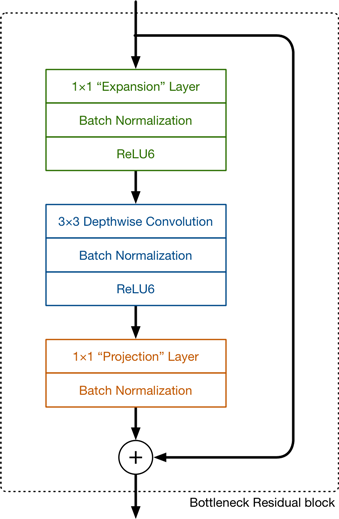
\includegraphics[scale = 0.5]{assets/ssdstruct1.png}
\caption{TODO: Saurabh}
\end{figure}

The first layer of the block is a 1×1 convolution. Its purpose is to expand the number of channels in the data before it goes into the depthwise convolution. Hence, this expansion layer always has more output channels than input channels. The second layer of the block is a depthwise convolution that filters the inputs. This is followed by a 1x1 pointwise convolutional layer which makes the number of channels smaller. This is why this layer is now known as the projection layer — it projects data with a high number of dimensions (channels) into a tensor with a much lower number of dimensions. For example, the depthwise layer may work on a tensor with 144 channels, which the projection layer will then shrink down to only 24 channels.

\begin{figure}[h!]
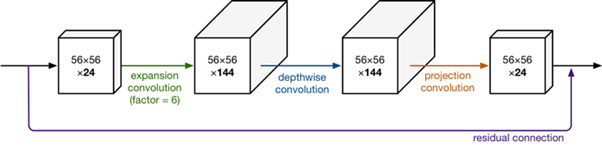
\includegraphics[width=\textwidth,keepaspectratio]{assets/ssdstruct2.png}
\caption{TODO:Saurabh}
\end{figure}

Then there is a residual connection that works just like in ResNet and exists to help with the flow of gradients through the network. The residual connection is only used when the number of channels going into the block is the same as the number of channels coming out of it, which is not always the case as every few blocks the output channels are increased. As usual, each layer has batch normalization and the activation function is ReLU6. This is like the well-known ReLU but it prevents activations from becoming too big:

\[  y = min(max(0,x),6)  \]

However, the output of the projection layer does not have an activation function applied to it. Since this layer produces low-dimensional data, using a non-linearity after this layer actually destroys useful information.
The full MobileNet V2 architecture, then, consists of 17 of these building blocks in a row. This is followed by a regular 1×1 convolution, a global average pooling layer, and a classification layer. (Small detail: the very first block is slightly different, it uses a regular 3×3 convolution with 32 channels instead of the expansion layer.)

\section{Model Deployment}

\subsection{Model Training}

Both models were trained on the KITTI dataset and an internal dataset given by CDAC Pune. The dataset was cleaned so as to remove all vehicles not annotated with the tag `Car'. However, it is possible to extend the same approach to multiple classes. Tiny YOLOv3 was trained on the official Darknet implementation, while SSD-Mobilenetv2 was trained with the Tensorflow Object Detection API.

The hyperparameters used for training can be found below:

\medskip

\begin{center}
\begin{tabular}{c|cc}
     & Tiny YOLOv3 & SSD Mobilenetv2 \\
    \hline
    Number of Layers & 23 & 53 \\
    Batch size & 16 & 16 \\
    Learning Rate & 0.001 & 0.002 \\
    Number of epochs & 13 & 12 \\
    Optimizer & ADAM & RMS Prop \\
    Number of classes & 1 & 1 \\
    Training data size & 5390 & 7156 \\
\end{tabular}
\captionof{table}{Hyperparameters for model training}
\end{center}

\subsection{Model Optimization}

While these trained models could immediately be used for real time inference. they would not give optimal performance, especially on resource constrained hardware like the Jetson Nano. This is where model optimization comes in. Model optimization can result in a decrease in size, latency, and memory usage. However, optimization can also result in changes to model accuracy, hence presenting a trade-off that needs to be considered in this part of the process.

\subsubsection{Model Quantization}

Model quantization reduces the precision of numbers used to represent a model's parameters, which is usually stored as a 32-bit floating point number (called FP32). This can reduce the size and speed of computation significantly, but could also affect accuracy. Models are usually quantized to either a 16-bit floating point number (FP16) or an 8-bit integer (INT8). The move from FP32 to FP16 can usually be done with insignificant loss of accuracy, but the conversion to INT8 is usually more complicated than that.

INT8 quantization compresses a 32 bit floating point number down to 8 bits. If we were to simply round the floating point number to an integer, this loss in precision would result in a massive degradation in accuracy, rendering it almost useless. Instead, the 32-bit values are mapped to 8 bit integer values. The candidates for the mapping are the inputs to each layer (activations), and the mapping is done by means of a linear mapping:

\[ T = sf \cdot t \]

where $T$ is the FP32 tensor,

$sf$ is a scaling factor,

$t$ is the INT8 tensor,

Sometimes, a bias term is also added, but it is normally not necessary.

To decide the scaling factor, we choose a threshold value $T$. All values outside the range $[-T,T]$ are given the extreme values of -127 or 127, and the values in between are linearly scaled to values between -127 and 127. Now, how do we decide the threshold $T$? Essentially, we are looking for a value of T that would minimize the difference between two distributions - the distribution of the FP32 tensors and the distribution of the INT8 tensors. The difference between them can be quantified using the Kullback-Leibler divergence. So, to choose the threshold $T$, we choose the value that minimizes the KL-divergence. This can be done by a simple iterative search for the right threshold value. 

Another important part of choosing the threshold value is the calibration dataset. The calibration dataset is ideally representative of the data that we expect to process, and it usually a subset of the validation dataset. It is used to generate histograms of activations from FP32 inference, from which multiple 8 bit representations are produced. The one with the least KL-divergence is chosen. This process is known as calibration.

\subsubsection{TensorRT}

TensorRT is an SDK developed by NVIDIA for high performance inference. Besides providing support for quantization, TensorRT can also be used to optimize Tensorflow models. It does this by providing platform dependent optimizations to certain Tensorflow subgraphs and operations with CUDA. By optimizing with TensorRT, we can obtain a speedup of over 800\%.

\subsubsection{Multithreading}

Both Tensorflow and Darknet speed up evaluation by using multiprocessing, which allows it to run on multiple CPU cores. We can get another small boost by using multi-threading. One thread (the producer) evaluates and image and produces bounding boxes, while a second thread (the consumer) takes these bounding boxes and uses OpenCV to draw it onto the video feed and write it to an output file (or video stream). It is important to note that the concurrency produced by multithreading is not ideal in Python, due to the Global Interpreter Lock.

\subsection{Model Deployment}

Once the models have been optimized, we need to deploy them for use. To do this, we used Flask - a Python web framework which can be used to create REST APIs. By wrapping our code in a Flask framework, we can create a web server, and send HTTP requests to process images or videos, and send the processed image or video with the bounding boxes back to the user. This makes it easier to use remotely, and more extensible - it is easy to interchange the currently used model with a new, more powerful model.

\section{Results}

\subsection{Evaluation Metrics}

Object detection models are evaluated using the metric of Mean Average Precision (MAP). To understand this metric, we must first understand the following terms:

\begin{enumerate}

    \item True Positive: A classification is a true positive when the IOU of the predicted bounding box and the ground truth bounding box is greater than some threshold, usually 0.5

    \item False Positive: A classification is a false positive if the IOU of the predicted bounding box and the ground truth is less than the threshold, or if it is a duplicate bounding box of another classification

    \item False Negative: A classification is a false negative if there is no detection at all, or if the predicted bounding box has an IOU above the specified threshold, but has the wrong classification.

    \item Precision: The ratio of the number of true positives to the total number of predicted positives is known as precision.
        \[ \text{Precision} = \frac{TP}{TP+FP} \]

    \item Recall: The ratio of the number of true positives to the total of ground truth positives is known as recall.
        \[ \text{Recall} = \frac{TP}{TP+FN}  \]

\end{enumerate}

By varying the confidence threshold on our bounding boxes, we are able to vary the precision and recall creating a curve called the Precision-Recall Curve (PR Curve). Using this curve, we are able to calculate the Average Precision (AP) of a class at a certain IOU threshold. This is defined as the mean of precisions at 11 equally spaced recalls. The mean of average precisions of all classes at all specified IOU thresholds is called the Mean Average Precision.

\subsection{Tiny YOLOv3}

\section{Future work}




\pagebreak

%%%%%%%%%%%%%%%%%%%%%%%%%%%%%%%%%%%%%%%%%%%%%%%%%%%%%%%%%%%%%%%%%%%%%%%%%%%%%%%

% Appendix A

\section*{Appendix A}
\label{sec:appa}
\addcontentsline{toc}{section}{\nameref{sec:appa}}

\begin{tabular}{|c | c|}
    \hline
    GPU & NVIDIA Maxwell architecture with 128 NVIDIA CUDA cores \\
    \hline
    CPU & Quad-core ARM Cortex A57 MPCore processor \\
    \hline
    Memory & 4GB 64-bit LPDDR4 \\
           & 1600 MHz-25.6GB/s \\
    \hline
    Storage & 16 GB eMMC 5.1 Flash \\
    \hline
    Video Encode & 250 MP/sec \\
                 & 1x 4K @ 30 (HEVC) \\
                 & 2x 1080p @ 60 (HEVC) \\
                 & 4x 1080p @ 30 (HEVC) \\
    \hline
    Video Decode & 500 MP/sec \\
                 & 1x 4K @ 60 (HEVC) \\
                 & 2x 4K @ 30 (HEVC) \\
                 & 4x 1080p @ 60 (HEVC) \\
                 & 8x 1080p @ 30 (HEVC) \\
    \hline
    Camera & 12 lanes (3x4 or 4x2) MIPI CSI-2 DPHY 1.1 (18 Gbps) \\
    \hline
    Connectivity & WiFi requires external chip \\
                 & 10/100/1000 BASE-T Ethernet \\
    \hline
    Display & HDMI 2.0 or DP1.2 , eDP 1.4 , DSI (1x2) 2 simultaneous \\
    \hline
    UPHY & 1 x1/2/4 PCI-e, 1x USB 3.0, 3x USB 2,0 \\
    \hline
    I/O & 1x SDIO / 2x SPI / 4x 12C / 2x I2S / GPIOs \\
    \hline
    Size & 69.6 mm x 45 mm \\
    \hline
    Mechanical & 260-pin edge connector \\
    \hline
\end{tabular}

\pagebreak

%%%%%%%%%%%%%%%%%%%%%%%%%%%%%%%%%%%%%%%%%%%%%%%%%%%%%%%%%%%%%%%%%%%%%%%%%%%%%%%

% References

\section*{References}
\label{sec:refer}
\addcontentsline{toc}{section}{\nameref{sec:refer}}


\pagebreak

%%%%%%%%%%%%%%%%%%%%%%%%%%%%%%%%%%%%%%%%%%%%%%%%%%%%%%%%%%%%%%%%%%%%%%%%%%%%%%%

% Glossary

\section*{Glossary}
\label{sec:glossary}
\addcontentsline{toc}{section}{\nameref{sec:glossary}}

\textbf{Bounding Box} A bounding box is a box that defines the dimensions of a box that surrounds the object being detected.

\noindent \textbf{Feature Extraction} Feature extraction is the reduction of raw data into a set of smaller, more easily describable features.

\noindent \textbf{K means Clustering} K-means clustering is a clustering algorithm that partitions observations into k clusters, where each observation belongs to the cluster with the nearest mean, which serves as the prototype of the cluster.

\noindent \textbf{Loss Function} The loss function is a function that maps variables or values to a single real number that represents the “cost” associated with that set of values. In neural networks, it is an indicator of how “good” a neural network is.

\noindent \textbf{Sigmoid function} The sigmoid function is a class of functions that has a range from [0,1] and has a characteristic S-shaped curve.

\noindent \textbf{KL-divergence}

\noindent \textbf{HTTP}

\noindent \textbf{REST}

\pagebreak

\end{document}

